\section{Metodologia}\label{metodologia}

Apresenta-se a seguir o enquadramento metodológico adotado neste trabalho. Para organizá-lo, utilizou-se como referência o modelo de \citeonline{Wohlin2024}, que estrutura as decisões de uma pesquisa em três fases (estratégica, tática e operacional), partindo da questão de pesquisa e chegando aos achados. A Figura \ref{fig:enqmetodologia} apresenta o enquadramento deste estudo, em que os elementos destacados correspondem às escolhas adotadas.

\begin{figure}[h!]
    \caption{Enquadramento metodológico do estudo}
    \centering
    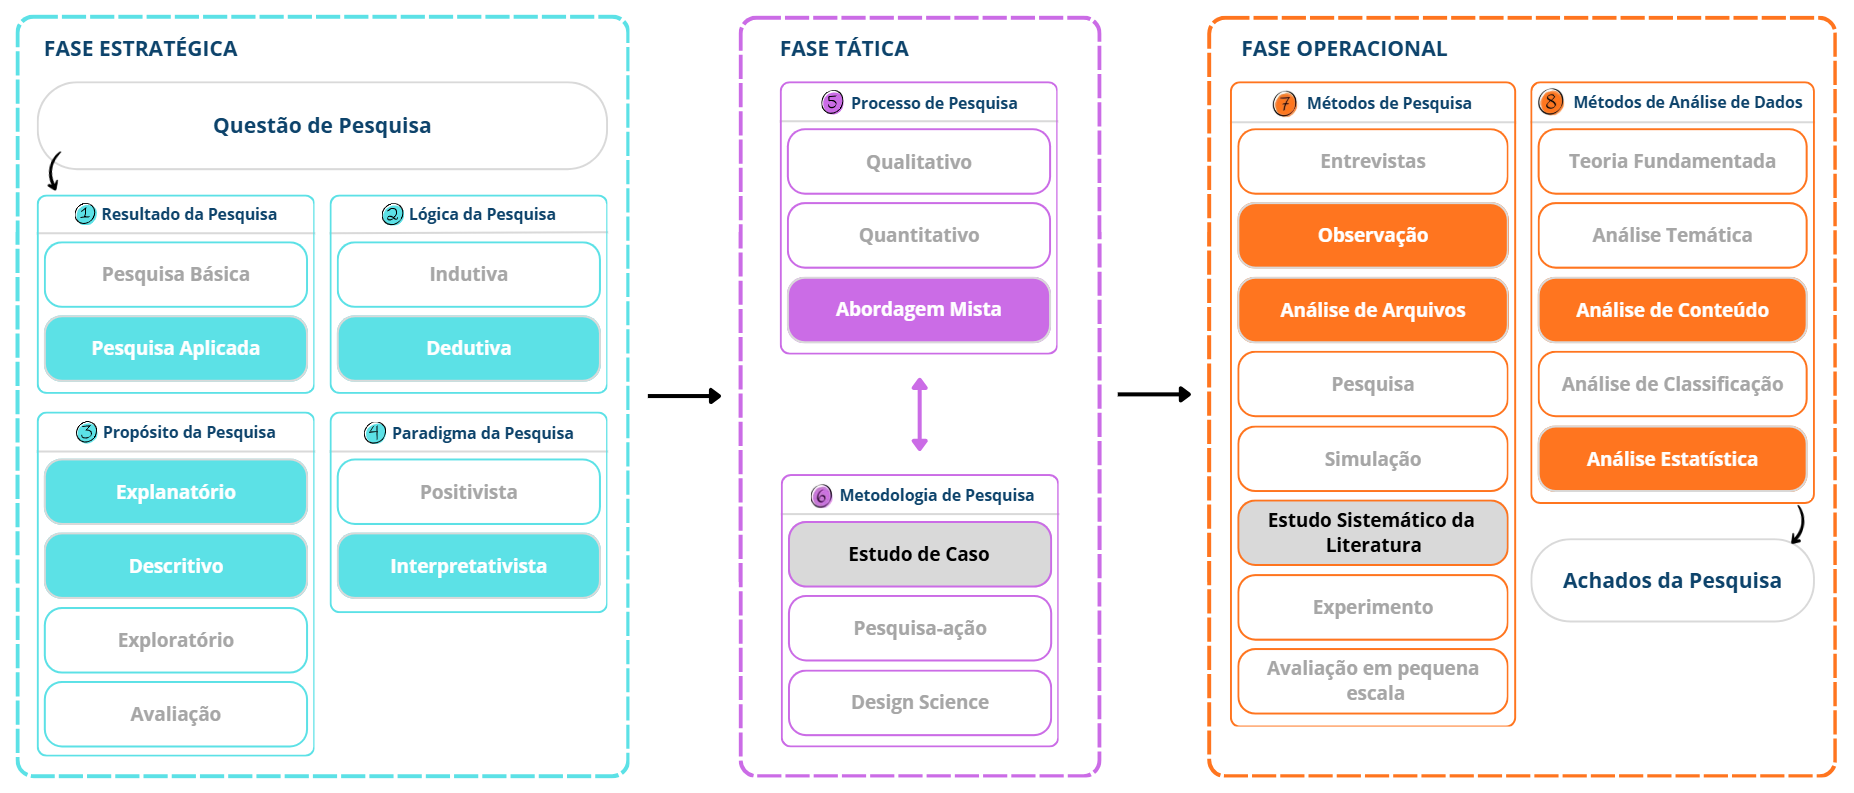
\includegraphics[width=1\linewidth]{figuras/metodologia.png}
    \caption*{Fonte: Adaptado de \citeonline{Wohlin2024}}
    \label{fig:enqmetodologia}
\end{figure}

Na \textit{fase estratégica}, a questão de pesquisa \ref{sec:questao} conduz a uma pesquisa aplicada, pois busca orientar a escrita de especificações BDD com vistas ao uso prático na geração de testes automatizados. A lógica é dedutiva, já que parte de conceitos consolidados na literatura, como a \cite{ISO25010}, o BDD e a AI aplicada a testes, para examinar um caso concreto. O propósito é descritivo e explanatório: descreve-se como as especificações BDD são estruturadas e explica-se como essa estruturação influencia a interpretação por sistemas de AI. O paradigma é interpretativista, pois o estudo busca compreender o fenômeno em seu contexto real, a partir da interpretação dos artefatos do projeto e do código gerado, com as métricas quantitativas servindo de apoio a essa interpretação.

Na \textit{fase tática}, adota-se uma abordagem mista, que combina a análise qualitativa das especificações e da literatura com a análise quantitativa de métricas de eficácia e qualidade do código gerado. A metodologia segue o protocolo de estudo de caso \cite{runeson_case_study_2012,yin_case_study_2009}, em um estudo observacional retrospectivo de caso único. Na \textit{fase operacional}, os métodos de pesquisa são a observação e a análise de arquivos, isto é, as histórias de usuários do ZenHub e o repositório do projeto CAPJu, além da revisão estruturada da literatura. Os dados são tratados por análise de conteúdo e análise estatística descritiva. O detalhamento do protocolo está nos Capítulos \ref{ch:revisao} e \ref{ch:proposta}.

\subsection{Uso de Inteligência Artificial Generativa}

Durante a elaboração deste trabalho, utilizaram-se ferramentas de inteligência artificial generativa ChatGPT da \citeonline{openai2026chatgpt} (versão GPT-5.3), o Claude da \citeonline{anthropic2026claude} (família Claude 5.5 / Opus 5.5) e o Gemini da \citeonline{google2026gemini}, onde o emprego dessas tecnologias deu-se exclusivamente como suporte para revisão gramatical, o aprimoramento da clareza textual e a organização de tópicos. Destaca-se que o Claude foi utilizado para auxiliar na escrita das regras do System Prompt, para consultar a arquitetura do CAPJu, e em sua execução localmente. 